%%
\chapter{Domain modeling and monitoring goal definition in EMF and \viatra{}}
%%

In this chapter the creation of initial artifacts is presented: domain models and graph patterns.
Domain modeling is an essential part of our framework, as the domain model defines the structure of the runtime live model, and affects the whole process. 
After the domain model is known, graph pattern can be specified, which will be used later in runtime analysis.
In the framework domain modeling are technologically backed up by EMF (Eclipse Modeling Framework), 
while graph pattern definition and processing are provided by \viatra{}.

\section{Eclipse Modeling Framework}


\begin{figure}
	\begin{center}
		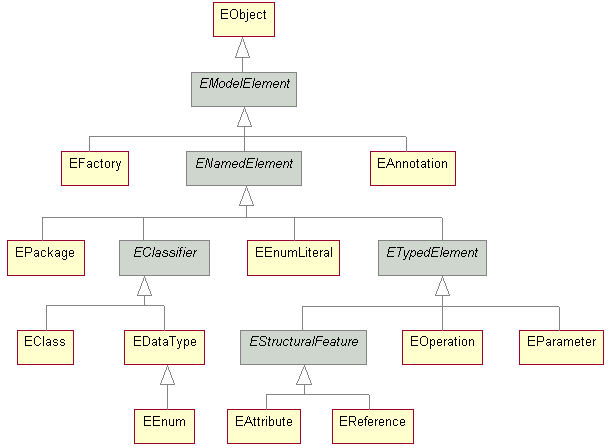
\includegraphics[width=0.5\textwidth]{figures/EcoreHierarchy.png}
		\caption{Hierarchy of Ecore elements (Source: \cite{ecore-package}) }
		\label{fig:ecore-hierarchy}
	\end{center}
\end{figure}

\begin{figure}
	\begin{center}
		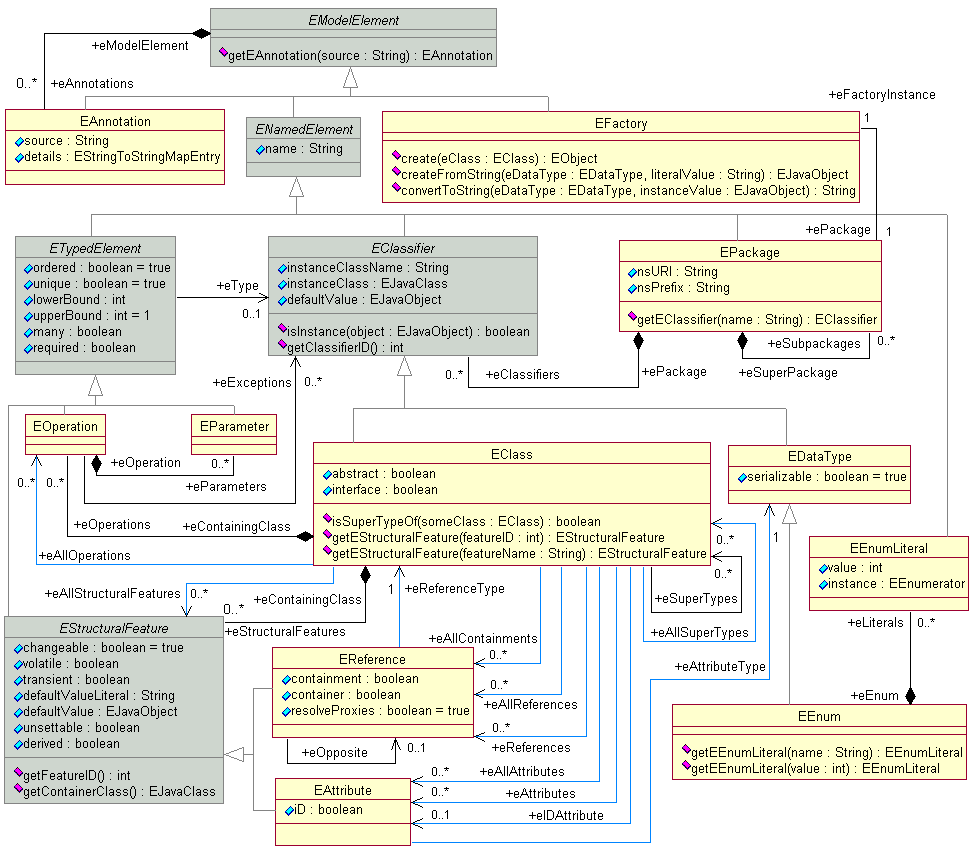
\includegraphics[width=\textwidth]{figures/EcoreRelations.png}
		\caption{Relations between Ecore elements (Source: \cite{ecore-package}) }
		\label{fig:ecore-relations}
	\end{center}
\end{figure}

Eclipse Modeling Framework (EMF) is an Eclipse based technology, which provides tools for model based developement: 
Ecore \cite{ecore-package} for metamodeling (Ecore actually defines a meta meta-model for metamodeling), and various tools like java code generation from ecore models, etc.

Ecore metamodeling is highly similar to defining class diagrams in UML, however, 
Ecore is more suitable for data and structural modeling: Interfaces are not a part of it, even though it can be substituted by abstract classes, as multiple inheritance is supported.

The hierarchy of Ecore elements can be seen on figure \ref{fig:ecore-hierarchy}, while its structure on \ref{fig:ecore-relations}
EObject is a base for everything, and its main purpuse to define the containment hierarchy of the model. 
EObjects can contain each other in a strict tree structure, circular containments are not permitted.
EModelElement expands EObject by giving the possibility to annotate them.

An Ecore model contains packages (EPackage). 
Packages have a namespace URI (nsURI), which can be used to refer it in other context eg.\ Viatra graph pattern definition.
Packages can contain other subpackages, classes (EClass), enumerations (EEnum), and data types (EDataType).

Classes have structural features: references and attributes (EStructuralFeature, EReference, EAttribute); also they have operations (EOperation).
References and attributes have multiplicity, defining their lower and upper bound is also possible.
ECore also provides tools to define containment hierarchy in the domain model itself: References can be containment or containing reference (considering direction of the reference). 
Two way navigation can be achieved by defining two reference and set them as the EOpposite of each other. A reference cannot be the EOpposite of itself, but its not a problem in most of the cases (eg.: \texttt{Human} class and \texttt{Spuse} reference). 

Multiple inheritance is supported for classes (eSuperTypes refers to direct base classes, and eAllSuperTypes for all transitively inherited base classes).

Besides classes, packages can contain enumerations and data types. 
Basic data types -- like EString, EInt, EBoolean etc.\ -- are defined by EMF, so its mostly never necessary to define others.
Enumerations are consists of EEnumLiterals. 
EEnumLiterals have an integral unique value, and its name is encapsulated in its EEnumerator instance.


\section{\viatra{} query language (VQL)}

\todo{Itt magáról a viatráról is kell írni vagy valahol}

As stated before, graph patterns can be defined using \viatra{} query language (VQL). 
The language syntax is simple, altough complex queries are not always self evident how to be expressed.

\subsection{Pattern definition}
Patterns and its bodies can be given by the \emph{pattern} keyword. 
Parameters must be specified after the parameter name in round brackets. 
Bodies of the pattern are given in curly brackets, separeted by the \emph{or} keyword

\begin{minipage}{\textwidth}
\begin{lstlisting}[language=vql]
pattern patternName( p1: Type1, p2: Type2){
... // Constraints for first body
} or {
... // Constraints for second body
} ...
\end{lstlisting}
\end{minipage}


\subsection{Constraints}
Constraints are given like statements. 
Each constraint is followed by a semicolon.

\vspace{\abovedisplayskip}
\begin{minipage}{\textwidth}
Type constraint can be given by specifying the type, then the object in round brackets.
\begin{lstlisting}[language=vql]
pattern patternName( o ){
	Type(o);
}
\end{lstlisting}
\end{minipage}
\vspace{\belowdisplayskip}

\begin{minipage}{\textwidth}
Reference constraint can be given by specifying which type's which reference must be checked, then giving the source and target variables in round brackets:
\begin{lstlisting}[language=vql]
pattern patternName( p1: Person, p2: Person ){
	Person.friend(p1, p2);
}
\end{lstlisting}
\end{minipage}
\vspace{\belowdisplayskip}

\begin{minipage}{\textwidth}
Other patterns can be used as constraint with the find keyword:
\begin{lstlisting}[language=vql]
pattern patternName( p1: Type1, p2: Type2, p3: Type3 ){
	find otherPatternName(p1, p2);
	find otherPatternName(p2, p3);
}
\end{lstlisting}

Also we can use underscore instead of specifying parameters. 
This way the constraint is satisfied, if the pattern matches with anything in the place of underscores (existential quantification).
\begin{lstlisting}[language=vql]
pattern patternName( p1: Type1 ){
find otherPatternName(p1, _);
}
\end{lstlisting}

This is the same as the following (if x is not used anywhere else):
\begin{lstlisting}[language=vql]
pattern patternName( p1: Type1 ){
find otherPatternName(p1, x);
}
\end{lstlisting}
\end{minipage}
\vspace{\belowdisplayskip}

\begin{minipage}{\textwidth}
Negative application condition can be expressed by \texttt{neg find} keyword:
\begin{lstlisting}[language=vql]
pattern patternName( p1: Type1, p2: Type2 ){
	neg find otherPattern(p1, p2);
	Type1.reference(p1, p2);
}
\end{lstlisting}

Also, we can use underscore if we don't want that the other pattern match occurs with \emph{any} value at the underscores. ( ie.\ neg find can be used to express negated existential quantification along with negated expressions )

\begin{lstlisting}[language=vql]
pattern patternName( p1: Type1 ){
	neg find otherPattern(p1, _);
}
\end{lstlisting}

It is very important to clarify, that unlike in the case of find this is NOT the same as the following:

\begin{lstlisting}[language=vql]
pattern patternName( p1: Type1 ){
	neg find otherPattern(p1, x);
}
\end{lstlisting}
As this will match if there exist \emph{any} x, that (p1, x) not satisfies the otherPattern.


\end{minipage}
\vspace{\belowdisplayskip}





\begin{minipage}{\textwidth}
\texttt{count find} can be used to count maches to a given pattern ()
\begin{lstlisting}[language=vql]
pattern personPattern(p){
	Person(p)
}

pattern countPersons(cnt)
	cnt == count find personPattern(_);
}
\end{lstlisting}
	
\end{minipage}
\vspace{\belowdisplayskip}




\begin{minipage}{\textwidth}
The keyword check can be used to create a constraint, that a given java (XBase) expression is true. The expression only can refer to attribute  variables (Variables refering to data types instead of graph nodes).
\begin{lstlisting}[language=vql]
pattern adultPerson( p: Person ){
	Person.age(p, age);
	check(age >= 18);
}
\end{lstlisting}
\end{minipage}
\vspace{\belowdisplayskip}

\begin{minipage}{\textwidth}
The keyword eval can be used to evaluate a java (XBase) expression on attribute variables and assign the result to another variable.
\begin{lstlisting}[language=vql]
pattern patternName( p1: Person, p2: Person, agesum : EInt ){
	Person.age(P1, a1);
	Person.age(P2, a2);
	agesum = eval(a1 + a2);
}
\end{lstlisting}
\end{minipage}
\vspace{\belowdisplayskip}



\todo{ count find, equality, inequality}

\subsection{Annotations}

\begin{minipage}{\textwidth}
Annotations can be added to patterns with the following syntax:
\begin{lstlisting}[language=vql]
@AnnotationName(
	a = {p1, p3}
	a = {p2, p3}
	b = "A simple string"
)
@AnnotationName2
pattern patternName( p1, p2, p3, ... )
	...
\end{lstlisting}
\end{minipage}
\vspace{\belowdisplayskip}

An annotation has a name (after @), and some named attributes using \texttt{name = value} syntax inside parentheses.
One attribute name can used multiple times. 
The attribute's value can be a single value or a list of values, that can be strings, numerals, or parameter reference.


\subsubsection{Annotations used by our framework}

The framework can process two types of annotations:
\begin{itemize}
	\item \texttt{@Bind} can be used to control what kind of graph pattern matching code will be generated, ie.\ what parameter sets can be bind to restrict the results. The version of the query, where all the parameters are unbound are generated by default.
	
	\item \texttt{@SkipDefaultGen} can be used to avoid default query generation for unbound version, eg.\ in case of helper patterns, we would not want to use it by itself most of the time.
	
\end{itemize}


\section{VQL examples from the case study}

To show how the various vql elements can be used in patterns, now I present the benchmarked queries, and what their semantics are.

\subsection{\texttt{trainLocations}}
\begin{minipage}{\textwidth}
If we want all the train locations to be queriable we can use the following pattern. 
If we want to know a train's location a version is generated, where the user can bound the train parameter
\begin{lstlisting}[language = vql]
@Bind(
	parameters=train
)
pattern trainLocations(train: Train, loc: RailRoadElement)
{
Train.on(train, loc);
}
\end{lstlisting}
\end{minipage}
\vspace{\belowdisplayskip}




\subsection{\texttt{derailment}}
\begin{minipage}{\textwidth}
Derailment means, that on a turnout, the train is on the non-connecting element.
	
\begin{lstlisting}[language = vql]
pattern derailment(elem: RailRoadElement, train: Train)
{
Turnout(turnout);
RailRoadElement.train(elem,train);

neg find connected(elem, turnout);
find straightOrDivergent(turnout, elem);
}

// Helper pattern, does not need to be generated, if not used
@SkipDefaultGen
private pattern straightOrDivergent(turnout : Turnout, elem : RailRoadElement){
	Turnout.straight(turnout, elem);
} or {
	Turnout.divergent(turnout, elem);
}

// We need this query, because negation can be only be expressed with neg find
@SkipDefaultGen
private pattern connected(a : RailRoadElement, b : RailRoadElement){
	RailRoadElement.connectedTo(a,b);
}


\end{lstlisting}
\end{minipage}
\vspace{\belowdisplayskip}




\subsection{\texttt{closeTrains}}
\begin{minipage}{\textwidth}
Two trains are close, if they are on two segments that are connected by another segment
\begin{lstlisting}[language = vql]
pattern closeTrains(start : RailRoadElement, end : RailRoadElement)
{
	Train.on(t1,start);
	
	RailRoadElement.connectedTo(start,middle); // Has EOpposite, inverse navigation is effective even without model index
	RailRoadElement.connectedTo(middle, end);
	
	Train.on(t2, end);
	
	start != end; // This ensures that the start and end segment is different
	
	t1 != t2; // A train may occupy two neighboring segments when moving; this is not a hazardous situation
}
\end{lstlisting}
\end{minipage}
\vspace{\belowdisplayskip}




\subsection{\texttt{endOfSiding}}

End of siding pattern matches, when there is a last segment of railroad, and a trail is near to that segment.
The last segment is expressed as a segment, which has a neighbor, but only one.
If a train is on the neighbor, the pattern matches.

\begin{minipage}{\textwidth}
\begin{lstlisting}[language = vql]
pattern endOfSiding(train: Train, end: RailRoadElement, neighbor: RailRoadElement)
{
	RailRoadElement.train(neighbor, train);		
	RailRoadElement.connectedTo(end,neighbor);
	1 == count find connected(end,_);	
}


\end{lstlisting}
\end{minipage}
\vspace{\belowdisplayskip}


